\chapter{Use Cases}

This chapter presents three use cases of interactive visualization in the context of biomedical imaging using the \emph{slicevis} packge. All necessary datasets are included in the repository, as mentioned in the second chapter. 

\section{Whole-Body Murine CT Scans}
The first use case is a CT scan of a laboratory mouse. The image file is called \texttt{CT280.gff} and a corresponding organ segmentation is included as \texttt{CT280\_organs.segff}. Both files were published in an open access manner as part of a paper by Rosenhain et al. \cite{rosenhain}.

The combination of high-quality CT scan and labeled segmentations make this dataset quite suitable to showcase the capabilities of \emph{slicevis}. Due to the relatively small image size, the slices render quickly which makes the user interactions feel fluid. A validation segmentation is not required and hence not provided for this use case.

\begin{figure}[h]
	\centering
	\begin{subfigure}[t]{0.4\linewidth}
		\centering
		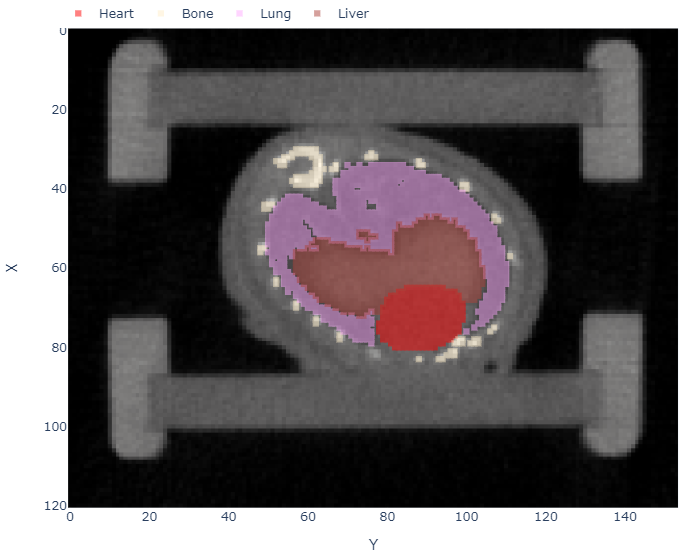
\includegraphics[width=\linewidth]{figures/mouse_axial.png}
		\caption{Axial slice.}
	\end{subfigure}
	\hfill
	\begin{subfigure}[t]{0.55\linewidth}
		\centering
		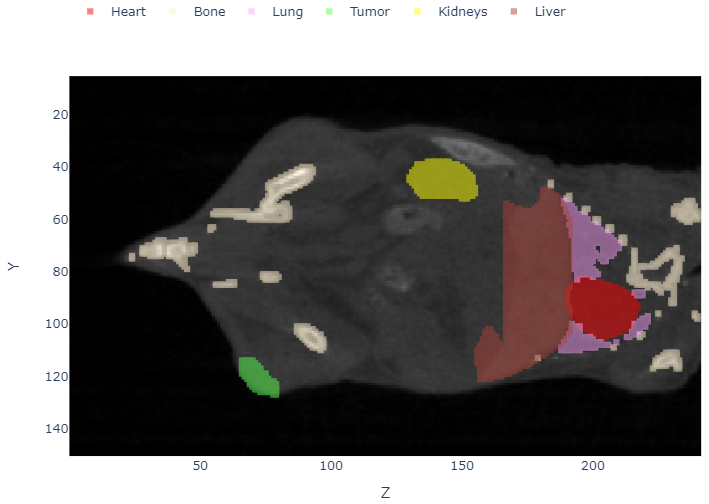
\includegraphics[width=\linewidth]{figures/mouse_coronal.png}
		\caption{Coronal slice.}
	\end{subfigure}
\end{figure}

\section{Lung Tumors}
The second example is a CT scan of a human upper body which was initially published by \emph{The Cancer Imaging Archive}. The file is title \texttt{lung.nii.gz} in the examples directory. It is part of a database to train machine learning models to detect lung cancer and it was republished as part of the \emph{Medical Segmentation Decathlon} under a CC-BY-SA license \cite{data}.

The scan is very high resolution and thus large in size (512 by 512 pixels in the axial slice) which makes slice visualization computationally more demanding.

Labels of lung nodules, segmented by trained radiologist, were also included in the dataset and the corresponding file for this case is \texttt{lung\_labels.nii.gz}. By loading both the image and label after each other in \emph{SliceWidget}, one can precisely locate the tumors, zoom in and visually evaluate the segmentation precision.

\begin{figure}[h]
	\centering
	\begin{subfigure}[t]{0.45\linewidth}
		\centering
		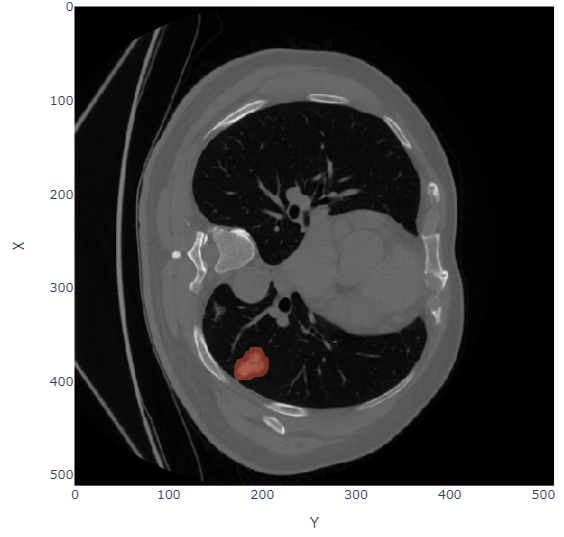
\includegraphics[width=\linewidth]{figures/lung_label.png}
		\caption{Axial slice with labeled tumor.}
	\end{subfigure}
	\hfill
	\begin{subfigure}[t]{0.45\linewidth}
		\centering
		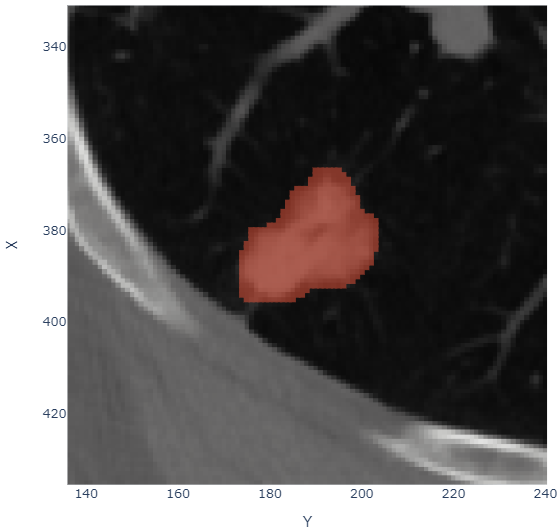
\includegraphics[width=\linewidth]{figures/lung_zoom.png}
		\caption{Zoomed in.}
	\end{subfigure}
\end{figure}

\section{nnU-Net Prediction}
The third example included in the repository is a prediction of lung tumors by a sophisticated convolutional neural network. The model is call nnU-Net and it was the winner of the Decathlon challenge \cite{nnunet}. It claims to have an average accuracy of 69\% for the lung task.

The file is called \texttt{lung\_prediciton.nii.gz} and it was created by downloading pre-trained model weights and executing a prediction on \texttt{lung.nii.gz}.

The aim is to visualize the prediction on top of the label and validate it using the DICE score (see \cref{eq:dice}). It is always automatically computed once a validation segmentation is loaded and displayed to the user.

\begin{figure}[h]
	\centering
	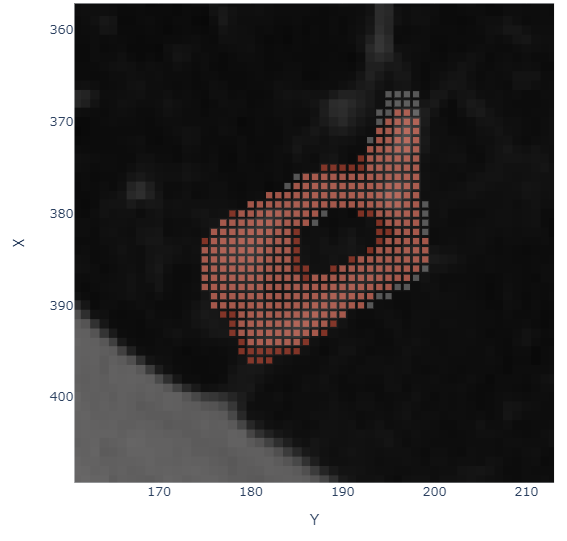
\includegraphics[width=.5\linewidth]{figures/lung_prediction.png}
	\caption{Lung tumor prediction (red) vs. label (white).}
	\label{fig:prediction}
\end{figure}

\Cref{fig:prediction} shows an exemplary zoomed-in slice of the validation. The white pixels are the label and the red ones are the prediction. In this slice, the prediction matches much better than expected and the overall score was computed to be approximately 96\%. But there are also cases where the model performs worse. Overall, this use case illustrates again that \emph{slicevis} is a very useful tool to interactively visualize and explore segmentations of medical images.